\documentclass{llncs}

% define general format 
\usepackage[margin=1.5in]{geometry}

% import req basic packages
\usepackage[dvipsnames]{xcolor}
\usepackage[tracking=true]{microtype}
\usepackage{amsmath, amssymb}
\usepackage{subcaption}
\usepackage{graphicx}
\usepackage{svg}
\usepackage{ifthen}
\usepackage{lineno}
\usepackage[utf8]{inputenc}
\usepackage[title]{appendix}

% tikz stuffs
\usepackage{tikz, tkz-orm, pgfplots}
\usetikzlibrary{arrows,shapes,automata,backgrounds,petri,decorations.markings}
\usetikzlibrary{matrix,positioning,decorations.pathreplacing,calc,tikzmark}
\pgfplotsset{width=7.5cm,compat=1.12}
\usepgfplotslibrary{fillbetween}

% customised links
\usepackage{hyperref}
\hypersetup{
    colorlinks,
    linkcolor={red!50!black},
    citecolor={blue!50!black},
    urlcolor={blue!80!black}
}


% code display style
\usepackage{verbatim}
\usepackage{listings}
\definecolor{codegreen}{rgb}{0,0.6,0}
\definecolor{codegray}{rgb}{0.5,0.5,0.5}
\definecolor{codepurple}{rgb}{0.38,0,0.52}
\definecolor{backcolour}{rgb}{0.95,0.95,0.95}

\lstdefinestyle{mystyle}{
    backgroundcolor=\color{backcolour},   
    commentstyle=\color{codegreen},
    keywordstyle=\color{codepurple},
    numberstyle=\tiny\color{codegray},
    stringstyle=\color{codepurple},
    basicstyle=\ttfamily\footnotesize,
    breakatwhitespace=false,         
    breaklines=true,                 
    captionpos=b,                    
    keepspaces=true,                 
    numbers=left,                    
    numbersep=5pt,                  
    showspaces=false,                
    showstringspaces=false,
    showtabs=false,                  
    tabsize=2
}

\lstset{style=mystyle}


\title{Big brain matrix eigenvalue lightspeed fourier transform for the great good solar light}

\subtitle{A 4-bit waltz in frequency space}

\author{Pushkar Mohile \texttt{(180260027)} \and Sankalp Gambhir \texttt{(180260032)}}
\institute{Indian Institute of Technology, Bombay}

\begin{document}
    \maketitle

    \begin{abstract}
    Identification of sounds has immense applications in the embedded systems space,
    ranging from simple detection of sounds to complete voice transcription. Being
    able to do this on low power devices is an area of active interest. We present a
    new approach to this problem involving bypassing a complete Fourier Transform
    and approximating its results using a cross-correlation based approach pruning a
    tree of (preset) frequencies. Our method returns present frequencies with
    reasonable accuracy whilst maintaining the speed expected of such an embedded
    system.
    \end{abstract}

    \section{Project Details}
        \subsection{Motivation}

\subsubsection{Why are Fourier Transforms imp?} Fourier transforms are the most important tools used in data processing. The relative amplitudes of the signal at different frequencies give us a lot of characterising data of the signal, and changing the signal in frequency space has a lot of applications, like auto-tuning, removing noise etc. The exact expression for a fourier transform is given by 
\begin{equation}
    \tilde{f}(\omega) = \int_{-\infty}^{\infty} e^{-i\omega t}f(t)
\end{equation}

\subsubsection{Fourier is Overkill.}
Looking at the structure of the Fourier transform, it is easy to see that it is
closely resembles the idea of a correlation, essentially extracting from the
signals its \emph{similarity} to a given frequency. These coefficients, gathered
using all frequencies, can produce a one to one mapping to a function space in
the frequency realm. However, the entire function is far too much information.
For most tasks involving categorization and identification of sounds,
fingerprinting is more than good enough. That is, considering the delta response
of the system, its restriction to a tiny subset of points in frequency space.

As such, simply extracting the info for these frequencies alone is sufficient,
and can be done whilst incorporating several statistical approximations. This is
easily done with a correlation of the signal with a pure mode. 

However, when frequencies are aggregated, the phase difference is absorbed into
the coefficients of multiple frequencies, but in the correlation scenario, no
such hope exists. This is where cross-correlation comes in. 

\begin{equation}
    (f \ast g)(t) \triangleq \int_{-\infty}^{+\infty} \overline{f(\tau)} \cdot g(t+\tau) d\tau
\end{equation}

By considering the similarities of shifted signals, we can infer more precise
information about their similarity in space, by completely disregarding the
temporal dimension. This is immensely useful in matching an externally sourced
wave of unknown phase with a synthetic mode of known or unknown phase to
identify the wave.

In particular, the global maximum of the cross-correlation may be taken as the
phase independent correlation of two signals.

\begin{equation}
    corr(f, g) \triangleq \max((f \ast g) (t))_t
\end{equation}
 % common

The main idea of this project is to extract some characteristic audio data from
the signal without having to resort to memory and computationally expensive
fourier transforms. The 2KiB SRAM of the Arduino is the biggest botleneck here
for doing any processing. In order to do this processing, we came up with
multiple optimizations. 

\subsection{Optimizations}

\subsubsection{Cross Correlations} 
Instead of doing a FFT on the data, we will extract a few characteristic
frequencies components by correlating the signal with a set of frequencies. The
expression for crosscorrelation of 2 discrete signals \(x,y\) is given by

\begin{equation}
    R_{xy}[k] = \sum_{i} x[i]y[i-k]
\end{equation}

Along with some normalization. The harmonics form a linearly independent set and
return zero-correlation when the product is integrated over several time periods,
i.e.

\begin{equation}
    \frac{1}{\pi} \int_0^{2\pi}sin(n_1x)sin(n_2x) = \delta_{nn'}  
\end{equation} 

Where \(\delta\) is the usual Kronecker delta. We can normalize the correlation
with the autocorrelation at 0 to get a number between -1 and 1 that
characterized the coeficients.

\begin{equation}
    c_{xy} = \frac{R_{xy}[0]}{\sqrt{R_{xx}[0]R_{yy}[0]} }
\end{equation} 

However, the above expression does not account for the phase shift \(\phi\)
between the harmonics which reduces the correlation by a factor of
\(cos(\phi)\)Therefore we modify check the signal with phase shifted test
harmonics by modifying the expression to:

\begin{equation}
    c_{xy} = \frac{\mathnormal{max}\{R_{xy}[k]\}}{\sqrt{R_{xx}[0]R_{yy}[0]} }
\end{equation}

This ensures that the loss due to potential phase shift is avoided by getting an
estimate of the phase. Further, these correlations avoid the complex
multiplications required in FFT calculations while giving more characteristic
data. 

\subsubsection{Memory Management}
We store the signal using an array of 4 bit numbers, i.e. numbers from -7 to 7.
This has multiple benefits, such as being able to outright store more numbers,
and more subtly, perform calculations in a smaller time period as the Arduino
processor is based around an 8-bit bus. Instead of requiring multiple clock
cycles to process 16 / 32 bit datatypes like \texttt{float} adn \texttt{int}, we
can process the signals much faster.

\subsubsection{Frequency Space Pruning}
Beginning with a Dirac comb in frequency space, we prune a lattice tree of the
frequency power set via depth first binary search. This bypasses the
computationally expensive cross correlation calculations for a lot of (wrong)
frequencies.  % common
\begin{figure}[ht]
    \centering
    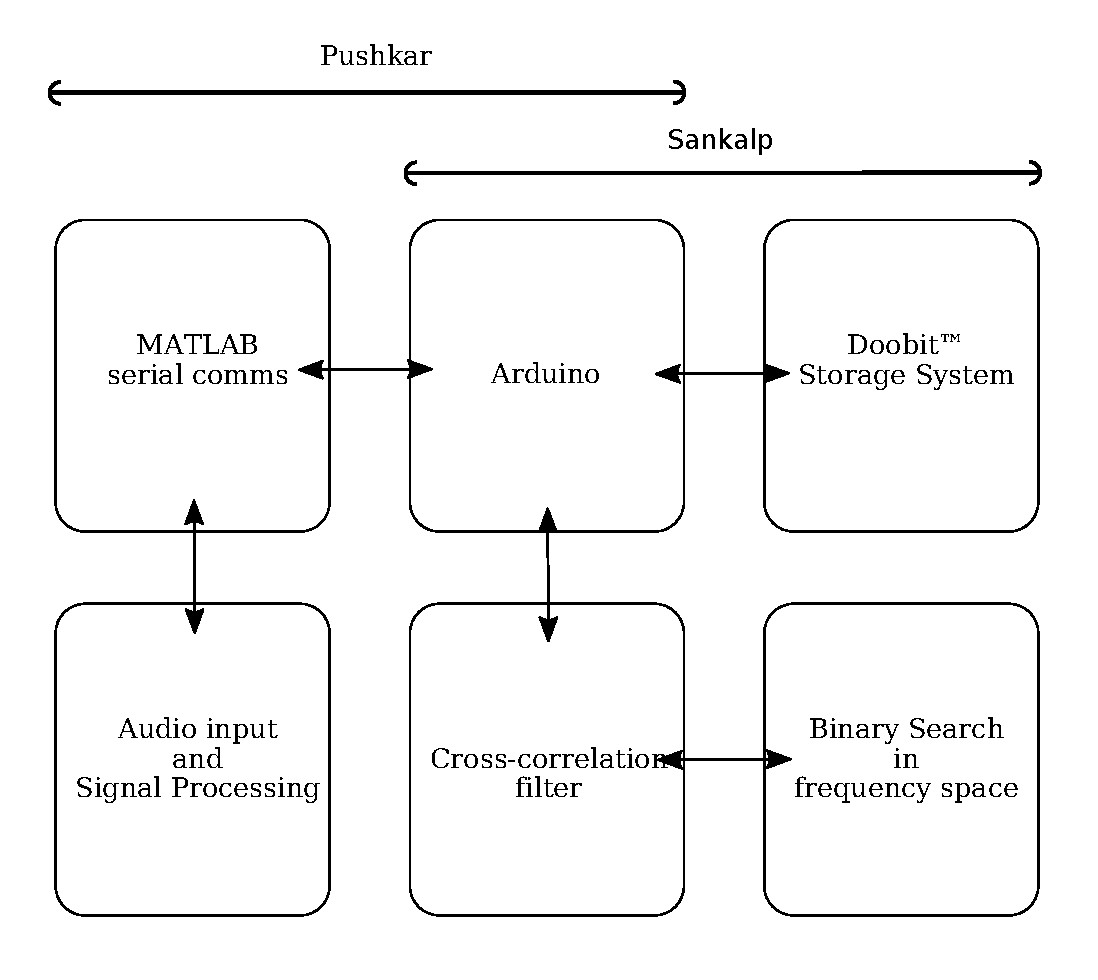
\includegraphics[height=0.4\textheight]{fig/blockdiag.pdf}
    \caption{Block diagram and work distribution.}
    \label{fig:blockdiag}
\end{figure}

% descrive blocks in brief % common
\subsection{Doobit™}

Working on the Arduino with signals very quickly turned into a constant battle
of resolution and storage, limited by its relatively tiny memory. After msot
optimizations we went through, managing memory manually very closely and
ensuring sequentialized execution contexts, we were teribly bottlenecked by the
storage. To work around this physical limit, we manage each byte of the stored
signal manually and instead of one, store two signal data points in every byte.
This reduces our data resolution by way of being limited to 4 bits, but grants
us unmatched robustness to noise by comparison, by doubling possible data
processing capabilities. The system has been affectionately named Doobit.

\begin{lstlisting}[language=C++]
// bit mask storage
struct doobit{
    uint_fast8_t data;

    doobit(int8_t x = 0, int8_t y = 0){ // handles all our casts too
        this->storelow(x);
        this->storehigh(y);
    }

    void storelow(int8_t);
    void storehigh(int8_t);

    int8_t getlow();
    int8_t gethigh();

    int16_t operator*(doobit& b);
};
\end{lstlisting}

A \texttt{struct} provides us fast access with very little memory and
performance overhead, something that only becomes more and more negligible as we
increase our (now doubled!) data numbers.

Unpacking the code block, \texttt{data} is the actual storage, an unsigned 8-bit
type, chosen this way to avoid accidental signed interpretation and any unwanted
processing by the compiler. Reliance on unsigneds in a case such as this is
common even within the compiler itself, where it would convert signeds to
unsigneds before evalutation to avoid ambiguity. In particular, a two's
complement could scramble the data beyond recognition quite quickly.

The \texttt{fast} part of \texttt{uint\_fast8\_t} indicates to the compiler that
we are looking for a type that is atleast 8 bits, but is the fastest among
those. On an Arduino Uno, of course, this is just the 8 bit unsigned integer,
but on more exotic embedded systems this could end up being a 9 or 10 bit type,
if not more. This notation allows for some compatibility between systems, though
as is with embedded systems, one would try to create more efficient structures
that exploit the architecture of those systems.

The storage of the signal is handled by the \texttt{storelow()} and
\texttt{storehigh()} functions, which store data into the 4 least significant
and 4 most significantbits of the storage \texttt{data} respectively. We look at
one of the functions:

\begin{lstlisting}[language=C++]
void doobit::storelow(int8_t x){
	this->data &= 0b11110000;  // clear for storage

	x += 7; // remove signed component
	assert((!(x & 0b11110000)) && "doobit range violation");

	this->data |= x;
}
\end{lstlisting}

This function takes in a value \texttt{x}, to be stored in the lower 4 bits of
\texttt{data}, and preparing for it, clears the lower 4 bits via an \texttt{AND}
operation with a bitmask \texttt{11110000}. Following this, a manual conversion
is made to ensure \texttt{x} is unsigned. The operation moves \texttt{x}'s
previous range, -7 to +7, to now 0 to 14, with 15 remaining generally unused,
rushing to somehow occupy this position leads to little benefit and after much
trial to squeeze extra storage out of the system, was abandoned. 

The \texttt{assert} exists merely for testing purposes to ensure our data can
indeed fit in 4 bits. Finally, having ensured \texttt{x} has only its lower bits
populated, an \texttt{OR} operation with the storage inserts it in.

The \texttt{storehigh()} function works in a similar manner, albeit with a bit
shift and an inverted bit mask to work on the 4 higher bits.

Now remains the issue of retrieving data from this storage, and is done as very
much the inverse of how it is stored:

\begin{lstlisting}[language=C++]
int8_t doobit::getlow(){
    int8_t x = (data & 0b00001111); // bitmask
    return (x-7); // reinsert sign
}
\end{lstlisting}

The \emph{unrequired} data is removed via a bit mask, and would be moved
rightwards via a bit shift in the case of \texttt{gethigh()}, and its signed
nature is restored by shifting it back to the original range.

The conversion to unsigned is quite important to have to not manage the carry
bits arising from a two's complement operation. The number -7 in C++ could
ambiguously be coming from an \texttt{int} (internally \texttt{int32\_t}) in
which case the signed bit is the 32nd, while it could also be coming from an 8
or 16 bit type, making the signed bit unclear and its extraction slow and
painful. Asking for a change of range was the fastest of the operations we
tested, included several bitwise only operations.

The storage could be optimized for several arithmetic operations, but for our
case in particular, for the correelation setups, we need only multiplication. As
of now, this is done simply by retrieving the numbers individually and
multiplying them pairwise. This is done as opposed to attempting bitwise
operations as (1), multiplication operations are quite optimized on a circuit
level in modern processors anyway, and more importantly (2), 4 bit being such a
limited storage type, would cause an overflow for most possible multiplication
operands.

\begin{lstlisting}[language=C++]
int16_t operator*(doobit& b){
    auto highprod = this->gethigh() * b.gethigh();
    auto lowprod = this->getlow() * b.getlow();
    return (highprod + lowprod);
}
\end{lstlisting}

This definition is obviously not compatible with all arithmetic operations, but
quite specific for our limited operations, kept this way to prevent
overcomplication of the rather heavily utilized routine.

The full code for all the functions may as always be found
\hyperref[sec:arduinocode]{in the Appendix}. % sankalp
\subsection{Serial Communication and the Great Horse Race}
The input of the system is handled using MATLAB. This is appealing for several
reasons, (1), we can immedietly visualise and process the sound array that we
get, making it easy to debu, and (2), we can use the inbuilt system microphone.
MATLAB by default offers several different ways to get this audio data, the
lowest resolution being a 1000Hz Sampling frequency and 8-bit sampling, using
the \texttt{audiorecorder} object. Once we record the relevent sample, we
extract an array with this data and after doing some basic filtering, to remove
any high frequency noise that may affect the signal, we send the data to the
Arduino via the Serial port. 

The important part here is understanding how the serial communication with the
Arduino works. The serial port can only send data character by character to the
Arduino and waits for it to be processed. Therefore the processing of the
integers is done as follows: 

\begin{enumerate}
    \item Collect multiple audio samples from the microphone. We take 2000
    datapoints, assuming a periodic sample. The points are all \texttt{int8}.

    \item Apply a filter to remove any peaks above \(\pm7\) to ensure that the
    data doesn't overflow in the arduino. Then we apply a Moving average filter
    by taking 3 200-datapoint samples from the 2000 datapoints to remove any
    anamolous noise in the data.

    \item In order to communicate this data, we convert the integer Array in
    MATLAB to strings using the \texttt{int2str} method so that it can be sent
    via the Serial port. The terminator that we use is the newline character
    '$\backslash$n'.

    \item We open the serial monitor and send the data character by character
    using the \texttt{fprintf} function in Matlab.

    \item We check for available data in the Arduino using the
    \texttt{Serial.available()} function.

    \item Then we read the data into an array in Arduino using the
    \texttt{Serial.parseInt()} function. We wait for 2 bytes to arrive and store
    them in a single byte on the arduino to work with our processing scheme.
    
    \item When all the expected data (200 points) are read, stop recording and
    do the processing to find the matching frequencies. 

    \item Send the frequencies back to MATLAB to print using the Serial port. 
\end{enumerate}

However, we ran into some issues here, where several values were not detected by
the Arduino. We tried multiple approaches to solve this 

\begin{enumerate}
    \item We increased the Baud rate to 115200 to ensure that the transmission
    wasn't causing any loss of data. 

    \item We added a small delay of 30ms between subsequent transmissions to
    ensure that the Arduino had time to process the data.

    \item The Serial protocol has a buffer that stores the incoming values
    before they are processed by the Arduino. In the Arduino Uno, this
    \texttt{SERIAL\_RX\_BUFFER} memory that stores the incoming data from the
    Serial Port is only 64 bytes. We changed the header files to make the buffer
    128 bytes in HardwareSerial.h so that more characters could be stored
    without losing them in transmission.
\end{enumerate}

In order to ensure that this method is working correctly we have several checks 

\begin{enumerate}
    \item We ran a simple program that turns the pin13 LED On and Off based on
    whether the character it received was 0 or -7.

    \item In our main code, pin 13 is HIGH when waiting for data and recording.
    When all the expected data has been found, it stops glowing.
    
    \item We also plot the raw data that we get from the Mic to ensure that a
    reasonable waveform has been detected.
\end{enumerate}

The code for testing the glowing of the LEDs is found here: 

\begin{lstlisting}[language=C++]
const int led = 13;
String text;
int k;
void setup() {
                //pinMode(led, OUTPUT);
                Serial.begin(9600);
                k = 0;
}
void loop() { 
  if (Serial.available()){
                    text = Serial.readStringUntil('$');
                    k = text.toInt(); 
                    if(k == -7){
                        digitalWrite(led, 1);
                    }
                    if(k == 0){
                        digitalWrite(led, 0);
                    }
  }
}
\end{lstlisting}

The MATLAB code for controlling this unit is found here: 

\begin{lstlisting}[language=Matlab]
Arduino = serial("COM4","BaudRate",9600);
fopen(Arduino) %This opens a monitor
fprintf(Arduino,'%s$',int2str(0));
fprintf(Arduino,'%s$',int2str(-7));
fclose(Arduino);
\end{lstlisting}

 % pushkar


    \section{Main components and Invectory}
        The project mainly revolves around processing onboard the Arduino, so not much hardware is required:

\begin{itemize}
    \item Arduino
    \item USB Cable for serial communication
    \item Mic -- replaced by laptop with MATLAB here
\end{itemize}

    \section{Results}
        \subsection{Synthetic Data}

First, tests were run on data generated in situ from a list of frequencies, coefficients, and phase differences

\begin{align*}
    c &= \{c_1, c_2, \ldots, c_n\}\\
    \omega &= \{\omega_1, \omega_2, \ldots, \omega_n\}\\
    \phi &= \{\phi_1, \phi_2, \ldots, \phi_n\}\\
\end{align*}

which generate a 'generating' function for the discrete signal to follow

\begin{align*}
    f(x) = \sum_{i = 1}^{n} c_i \cdot sin(w_i x + \phi_i)
\end{align*}

implemented as a lambda-function in code 

\begin{lstlisting}[language=C++]
auto f_gen = [w, c, p](int x){
                float sum = 0;
                for(int i = 0; i < wlist.size(); i++){
                    sum += c[i] * sin(w[i]*x + p[i]);
                }
                return 7.0*sum/float(std::accumulate(c.begin(), c.end(), 0));
            };
            
auto f = new signal[SIZE];

for(int x = 0; x < SIZE; x++){
    f[i] = signal(f_gen(2*x), f_gen(2*x + 1));
}
\end{lstlisting}

The normalising factor may be succinctly written as 

\begin{align*}
    a_N = \frac{7.0}{\sum_{i = 1}^{n}c_i}~.
\end{align*}

It simply ensures that the cross correlation of the signals do not blow up and
that a single signal agnostic threshold value may be chosen as a metric for
matching. The factor of 7 scales the float value to the range (-7, 7) so as to
maintain reasonable resolution after conversion to integer type to save memory.

The signal is generated as even/odd pairs to facilitate pairwise storage
implemented by \nameref{sec:doobit}. The typename \texttt{signal} is an alias
for \texttt{doobit}, kept as such for modularity amongst storage backends, and
to possibly expand across architectures, saving major edits.

Playing with the described parameters, experiments were performed, and the
results have been tabulated in \autoref{fig:synthexp}. Since we look for a
global maxima of cross correlation, the phase is irrelevant to the results, but
for the sake of completeness, an indication has been provided where phase shifts
were tested. Several arbitrary values were tested, with the result being
uneaffected as expected.

\begin{figure}[ht]
    \centering
    \def\arraystretch{1.5}
    \setlength\tabcolsep{2em}
    \begin{tabular}{c | c | c}
        NCC Threshold (t)   & Input frequencies and coefficients (kHz)      & Output (kHz)  \\ \hline
        0.1                 & 0.3, 0.5, 0.8                                 & 0.3, 0.5, 0.8 \\
        0.1                 & 0.3, 0.5, 0.8$^\dagger$                       & 0.3, 0.5, 0.8 \\
        0.1                 & 0.3, 0.5$^\dagger$, 0.8$^\dagger$             & 0.3, 0.5, 0.8 \\
        0.2                 & 0.3, 0.5$^\dagger$, 0.8$^\dagger$             & 0.3, 0.5, 0.8 \\
        0.2                 & 0.3, 0.5$^\dagger$, 0.8$^\dagger$             & 0.3, 0.5, 0.8 \\
        0.2                 & 0.3, 4$\times$ 0.5$^\dagger$, 0.8$^\dagger$   & 0.3, 0.5, 0.8 \\
        0.4                 & 0.3, 4$\times$ 0.5$^\dagger$, 0.8$^\dagger$   & 0.3, 0.5, 0.8 \\
        0.5                 & 0.3, 4$\times$ 0.5$^\dagger$, 0.8$^\dagger$   & 0.3, 0.5      \\
        0.6                 & 0.3, 4$\times$ 0.5$^\dagger$, 0.8$^\dagger$   & 0.5           \\
        0.8                 & 0.3, 4$\times$ 0.5$^\dagger$, 0.8$^\dagger$   & $\emptyset$   \\
        0.1                 & 0.3, 0.5, 0.35$^\dagger$                      & 0.3, 0.4, 0.5 \\
        0.2                 & 0.3, 0.5, 0.35$^\dagger$                      & 0.3, 0.5     
    \end{tabular}
    \captionsetup{justification=centering}
    \caption{Experiments with varying synthetic inputs and thresholds.\\
    $\dagger.$ Phase shifted. Weight unit unless otherwise specified}
    \label{fig:synthexp}

\end{figure}

\subsection{Real Inputs}

Not having a microphone module for the Arduino, we resorted to passing a
recorded array to the device via MATLAB, opening its own can of worms by way of
buffer overflows and race conditions, as described in detail in
\autoref{subsec:buffinp}. 

For currently unknown reasons, we had memory overflows with the same size of
real data as we ran synthetic tests for. Curiously, in this case, the Arduino
continuosly prints \texttt{'w'} on the Serial line. After much testing we have
linked this behaviour to memory overflow, but are yet to find resources
confirming it. 

Reducing the size, however, allows us to perform some tests, limited by the data
transfer speed as well, with the serial line taking up to 30 seconds to transfer
all the data successfully, yet with significant packet loss. The best transfer
ratio we were able to obtain after fine tuning the transfer rates and timing was
400 packets received for 420 sent, but at this delicate parameter island, the
Arduino would, with roughly half probability, run out of memory. It may be
dependent on buffering of incoming packets. Buffering just a few more packets
may have been pushing it over the edge.

\begin{figure}[ht]
    \centering
    \def\arraystretch{1.5}
    \setlength\tabcolsep{2em}
    \begin{tabular}{c | c | c}
        NCC Threshold (t)   & Input signals                                 & Output (kHz) \\ \hline
        0.1                 & 0.4 kHz (generated using a phone speaker)     & INSERT \\   
        0.1                 & 0.5 kHz (generated using a phone speaker)     & INSERT \\   
        0.1                 & 0.6 kHz (generated using a phone speaker)     & INSERT \\   
        0.2                 & 0.6 kHz (generated using a phone speaker)     & INSERT \\   
        0.3                 & 0.6 kHz (generated using a phone speaker)     & INSERT \\   
        0.5                 & 0.6 kHz (generated using a phone speaker)     & INSERT \\   
        0.1                 & Speech                                        & INSERT \\   
        0.1                 & SOME SHIT CHORD                               & INSERT \\   
        0.1                 & SOME SHIT CHORD                               & INSERT \\   
        0.1                 & SOME SHIT CHORD                               & INSERT \\   
    \end{tabular}
    \captionsetup{justification=centering}
    \caption{Experiments with real inputs and thresholds.}
    \label{fig:realexp}

\end{figure}

screenshots of code compiled and running on arduino

photo video uploads

    \newpage
        
\begin{subappendices}
    \renewcommand{\thesection}{\Alph{section}}

    \section{Arduino Code}
    Here is the full code sent to the Arduino, verbatim.

    \lstinputlisting[language=C++]{../src/main.ino}
\end{subappendices}

\end{document}
